\def\CTeXPreproc{Created by ctex v0.2.14, don't edit!}\documentclass{beamer}
\usepackage{amssymb}
\usepackage{amsmath}
\usepackage{stmaryrd}
\usepackage{graphicx}
\usepackage{ctextemp_isabelle}
\usepackage{ctextemp_isabellesym}

\usepackage{ctex}

%%%%%%%%%%%% For Isabelle code
\newlength{\fminilength}
\newsavebox{\fminibox}
\newenvironment{fmini}[1][\linewidth]
  {\setlength{\fminilength}{#1\fboxsep-2\fboxrule}%
   \vspace{2ex}\noindent\begin{lrbox}{\fminibox}\begin{minipage}{\fminilength}%
   \mbox{ }\hfill\vspace{-2.5ex}}%
  {\end{minipage}\end{lrbox}\vspace{1ex}\hspace{0ex}%
   \framebox{\usebox{\fminibox}}}

\newenvironment{specification}
{\noindent\scriptsize
\tt\begin{fmini}\begin{tabbing}X\=X12345\=XXXX\=XXXX\=XXXX\=XXXX\=XXXX
\=\+\kill} {\end{tabbing}\normalfont\end{fmini}}

\usetheme{Warsaw}

\begin{document}

%%-------------------------------------------------

    \title{��е������֤���Լ�����ʽ����֤�е�Ӧ��}

    \author{���¼�}

    \institute{�������ѧ�����ص�ʵ����}

    \date{\today}

    \frame{\titlepage}

%%-------------------------------------------------

\begin{frame}\frametitle{Theorem prover(Proof assistant)}
\noindent
``A theorem prover is a computer program used interactively for developing human-readable reliable mathematical documents in a formal language."
\begin{itemize}
\item computer program (working mechanically)
\item interacting with people
\item a formal proof script as an output
\end{itemize}
\end{frame}

\begin{frame}\frametitle{Main Ideas}
\noindent
``A theorem prover is a computer program used interactively for developing human-readable reliable mathematical documents in a formal language."
\begin{itemize}
\item Formal logical calculus
\item Assistant people's formal logical calculus by a computer
\end{itemize}
\end{frame}


\begin{frame}\frametitle{Leibniz's opnion on formula logic }
``Leibniz enunciated the principal properties of what we now call conjunction, disjunction, negation, identity, set inclusion, and the empty set.
The principles of Leibniz's logic and, arguably, of his whole philosophy, reduce to two:"
\begin{itemize}
\item  All our ideas are compounded from a very small number of simple ideas, which form the alphabet of human thought.
\item Complex ideas proceed from these simple ideas by a uniform and symmetrical combination, analogous to arithmetical multiplication.
\end{itemize}
\end{frame}



\begin{frame}\frametitle{Theorem proving}
\vspace{2cm}
\begin{figure}[!ht]
% \centering %

\includegraphics[width=1.0\textwidth]{goal.pdf}
%\vspace{-0.5cm}
 \caption{Two figures}
\label{fig:arch}
\end{figure}

\end{frame}

\begin{frame}\frametitle{Main theorem provers}

\begin{itemize}
\item Isabelle
\item Coq
\item HOL4
\item PVS
\item .......
\end{itemize}
\end{frame}


\begin{frame}\frametitle{Main theorem provers}

\begin{figure}[!ht]
% \centering %

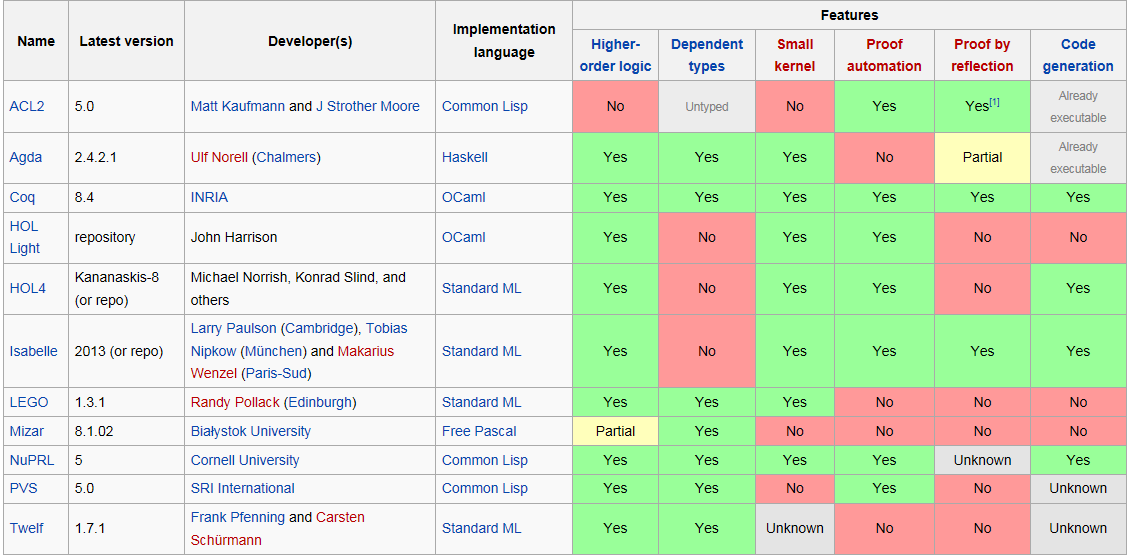
\includegraphics[width=1.0\textwidth]{thp.png}
%\vspace{-0.5cm}

\label{fig:arch}
\end{figure}
\end{frame}

\begin{frame}\frametitle{Use of theorem prover}

\begin{itemize}
\item Formalizing mathematics and mathematical libraries
\begin{itemize}
\item Mata theories: Set theory, LCF, ZF, ......
\item Some advanced theories: Kepler guess, Four-coloured problems

\end{itemize}
\item Formal verification of system (hardware design, program, algorithm, system)
\end{itemize}

\end{frame}

\begin{frame}\frametitle{The Kepler Conjecture}
\noindent
``The Kepler Conjecture says that the ?cannonball packing? (see picture) is a densest packing of 3-dimensional balls of the same size. This was stated as a fact by Kepler in 1611 but only proved by Thomas Hales in 1998. His proof relies on a Java program for generating all (3000) possible counterexamples (all of which are then shown not to be counterexamples). With the help of Isabelle we were able to prove the correctness of a functional implementation of his Java program. Listen to Thomas Hales speaking about the proof (ABC Radio National Science Show, March 11th 2006). A formal proof of the Kepler conjecture was completed in 2014."
\end{frame}

\begin{frame}\frametitle{Essentials of formal verification (by a theorem prover)}


\begin{itemize}
\item Formally model the system (by a  formula)
\item Formalize the specification (by a  formula)
\item Prove that the model satisfies the spec (logical deduction)
\end{itemize}
\end{frame}


\begin{frame}\frametitle{A case study---Formal verification of anonymity protocols (by a theorem prover)}


 \begin{specification}
 %\\
constdefs box::"agent$\Rightarrow$trace$\Rightarrow$trace set$\Rightarrow$
~~ assertOfTrace$\Rightarrow$bool" \\
~ "box A r rs Assert$\equiv$
 ~~$\forall$r'.r'$\in$rs$\longrightarrow$obsEquiv A  r r' $\longrightarrow$(Assert r')" \\

  \\
\\
constdefs diamond::"agent$\Rightarrow$trace$\Rightarrow$trace set$\Rightarrow$
  ~~ assertOfTrace$\Rightarrow$bool" \\
~ "diamond A r rs Assert$\equiv$
  ~~ $\exists$r'.r'$\in$rs
  $\wedge$obsEquiv A  r r'
~~ $\wedge$(Assert r')"
 \end{specification}


\end{frame}

\begin{frame}\frametitle{Formalization of anonymity properties}

\begin{specification}
constdefs senderAnomity::"agent set$\Rightarrow$agent$\Rightarrow$msg$\Rightarrow$\\
~~ trace$\Rightarrow$trace set$\Rightarrow$bool" \\
~ "senderAnomity AS B m r rs$\equiv$ ($\forall$X.X$\in$AS$\longrightarrow$
~~ r $\models \diamond$B rs (originates X m))"\\
\\


constdefs unlinkability::"agent set$\Rightarrow$agent$\Rightarrow$msg$\Rightarrow$ \\
~~ trace$\Rightarrow$trace set$\Rightarrow$bool" \\
~ "unlinkability AS A m r rs$\equiv$  \\
~~ (let P= $\lambda$X m' r. sends X m' r  in
~~ ($\neg$ (r $\models \box$ Spy rs (P A m)) $\wedge$ \\
~~ ($\forall$X.X$\in$AS $\longrightarrow$r
$\models \diamond$Spy rs (P A m)))"\\


\end{specification}

\end{frame}


\begin{frame}\frametitle{Modelling Onion Routing Protocols}
\begin{specification}
\\ --- Formal inductive definition
inductive\_set oneOnionSession::"nat$\Rightarrow$agent$\Rightarrow$trace set"\\
for k::"nat" and M::"agent" where \\
~ ~onionNil: "[]$\in$ (oneOnionSession k M) " \\
~ | onionCons1: "$\lbrakk$tr$\in$(oneOnionSession k M);X$\noteq$M;Y$\noteq$M;\\
~~ Nonce n0$\notin$(used tr);Nonce n$\notin$(used tr); \\
~~ length tr$<$k$\rbrakk$$\Longrightarrow$ \\
~~ Says X M (Crypt (pubK M) \\
~~  \lbrace Nonce n0,Agent Y,Crypt (pubK Y) (Nonce n)\rbrace) \\
~~ \#tr\in oneOnionSession k M"\\
~ | onionCons2: "$\lbrakk$tr$\in$(oneOnionSession k M);X$\noteq$M; \\
~~ Nonce n$\notin$(used  tr);length tr$<$k$\rbrakk$$\Longrightarrow$\\
~~ Says X M (Crypt (pubK M) (Nonce n)) \\
~~ \#tr\in oneOnionSession k M"\\

~ | onionCons3: "$\lbrakk$tr$\in$(oneOnionSession k M);\\
~~ length tr$\geq$k; \\
~~ Says M Y (Crypt (pubK Y) (Nonce n))\notin(set tr)$\rbrakk$\\
~~ $\Longrightarrow$Says M Y (Crypt (pubK Y) (Nonce n))\\
~~ \#tr\in oneOnionSession k M"
\end{specification}
\end{frame}


\end{document}
